\section{Equipment}\label{equipment}
The machine used for the measurement was a Keysight PNA N5527A 4-port VNA with parallel port capture and supports frequencies from 10MHz to 67 GHz.The VNA has a receiver $DR$ of 131dB. With a 4 port VNA the antennas can be set in a 1 TX and 3 RX configuration.This gives antenna diversity of 3. Calibration can be done by connecting the cables together and do a simple normalization. This normalization technique simplifies the calibration, but means a \gls{PA} can't be used.  The sweep data will be saved to a USB.


Cables used have a loss of $0.5dB  \ per \ m$. 3 10m cables and 1 4m cable for the RX and TX antennas respectively. This gives a total cable loss $L_c$ of 7dB.


The TX antenna is a directional antenna with a gain $G_{TX}=12.7dBi$ at 4.5GHz and $G_{TX}=10.7$ at 5.5GHz. The full gain chart of the antenna can be found in appendix \ref{ant_adix}.This difference will be accounted for during analysing of the data. The RX antenna array is a omnidirectional antenna with a 5Ghz $f_c$ and a spacing of $>0.4 \lambda$.

\begin{figure}[H]
  \centering
  \begin{minipage}[H]{0.42\textwidth}
    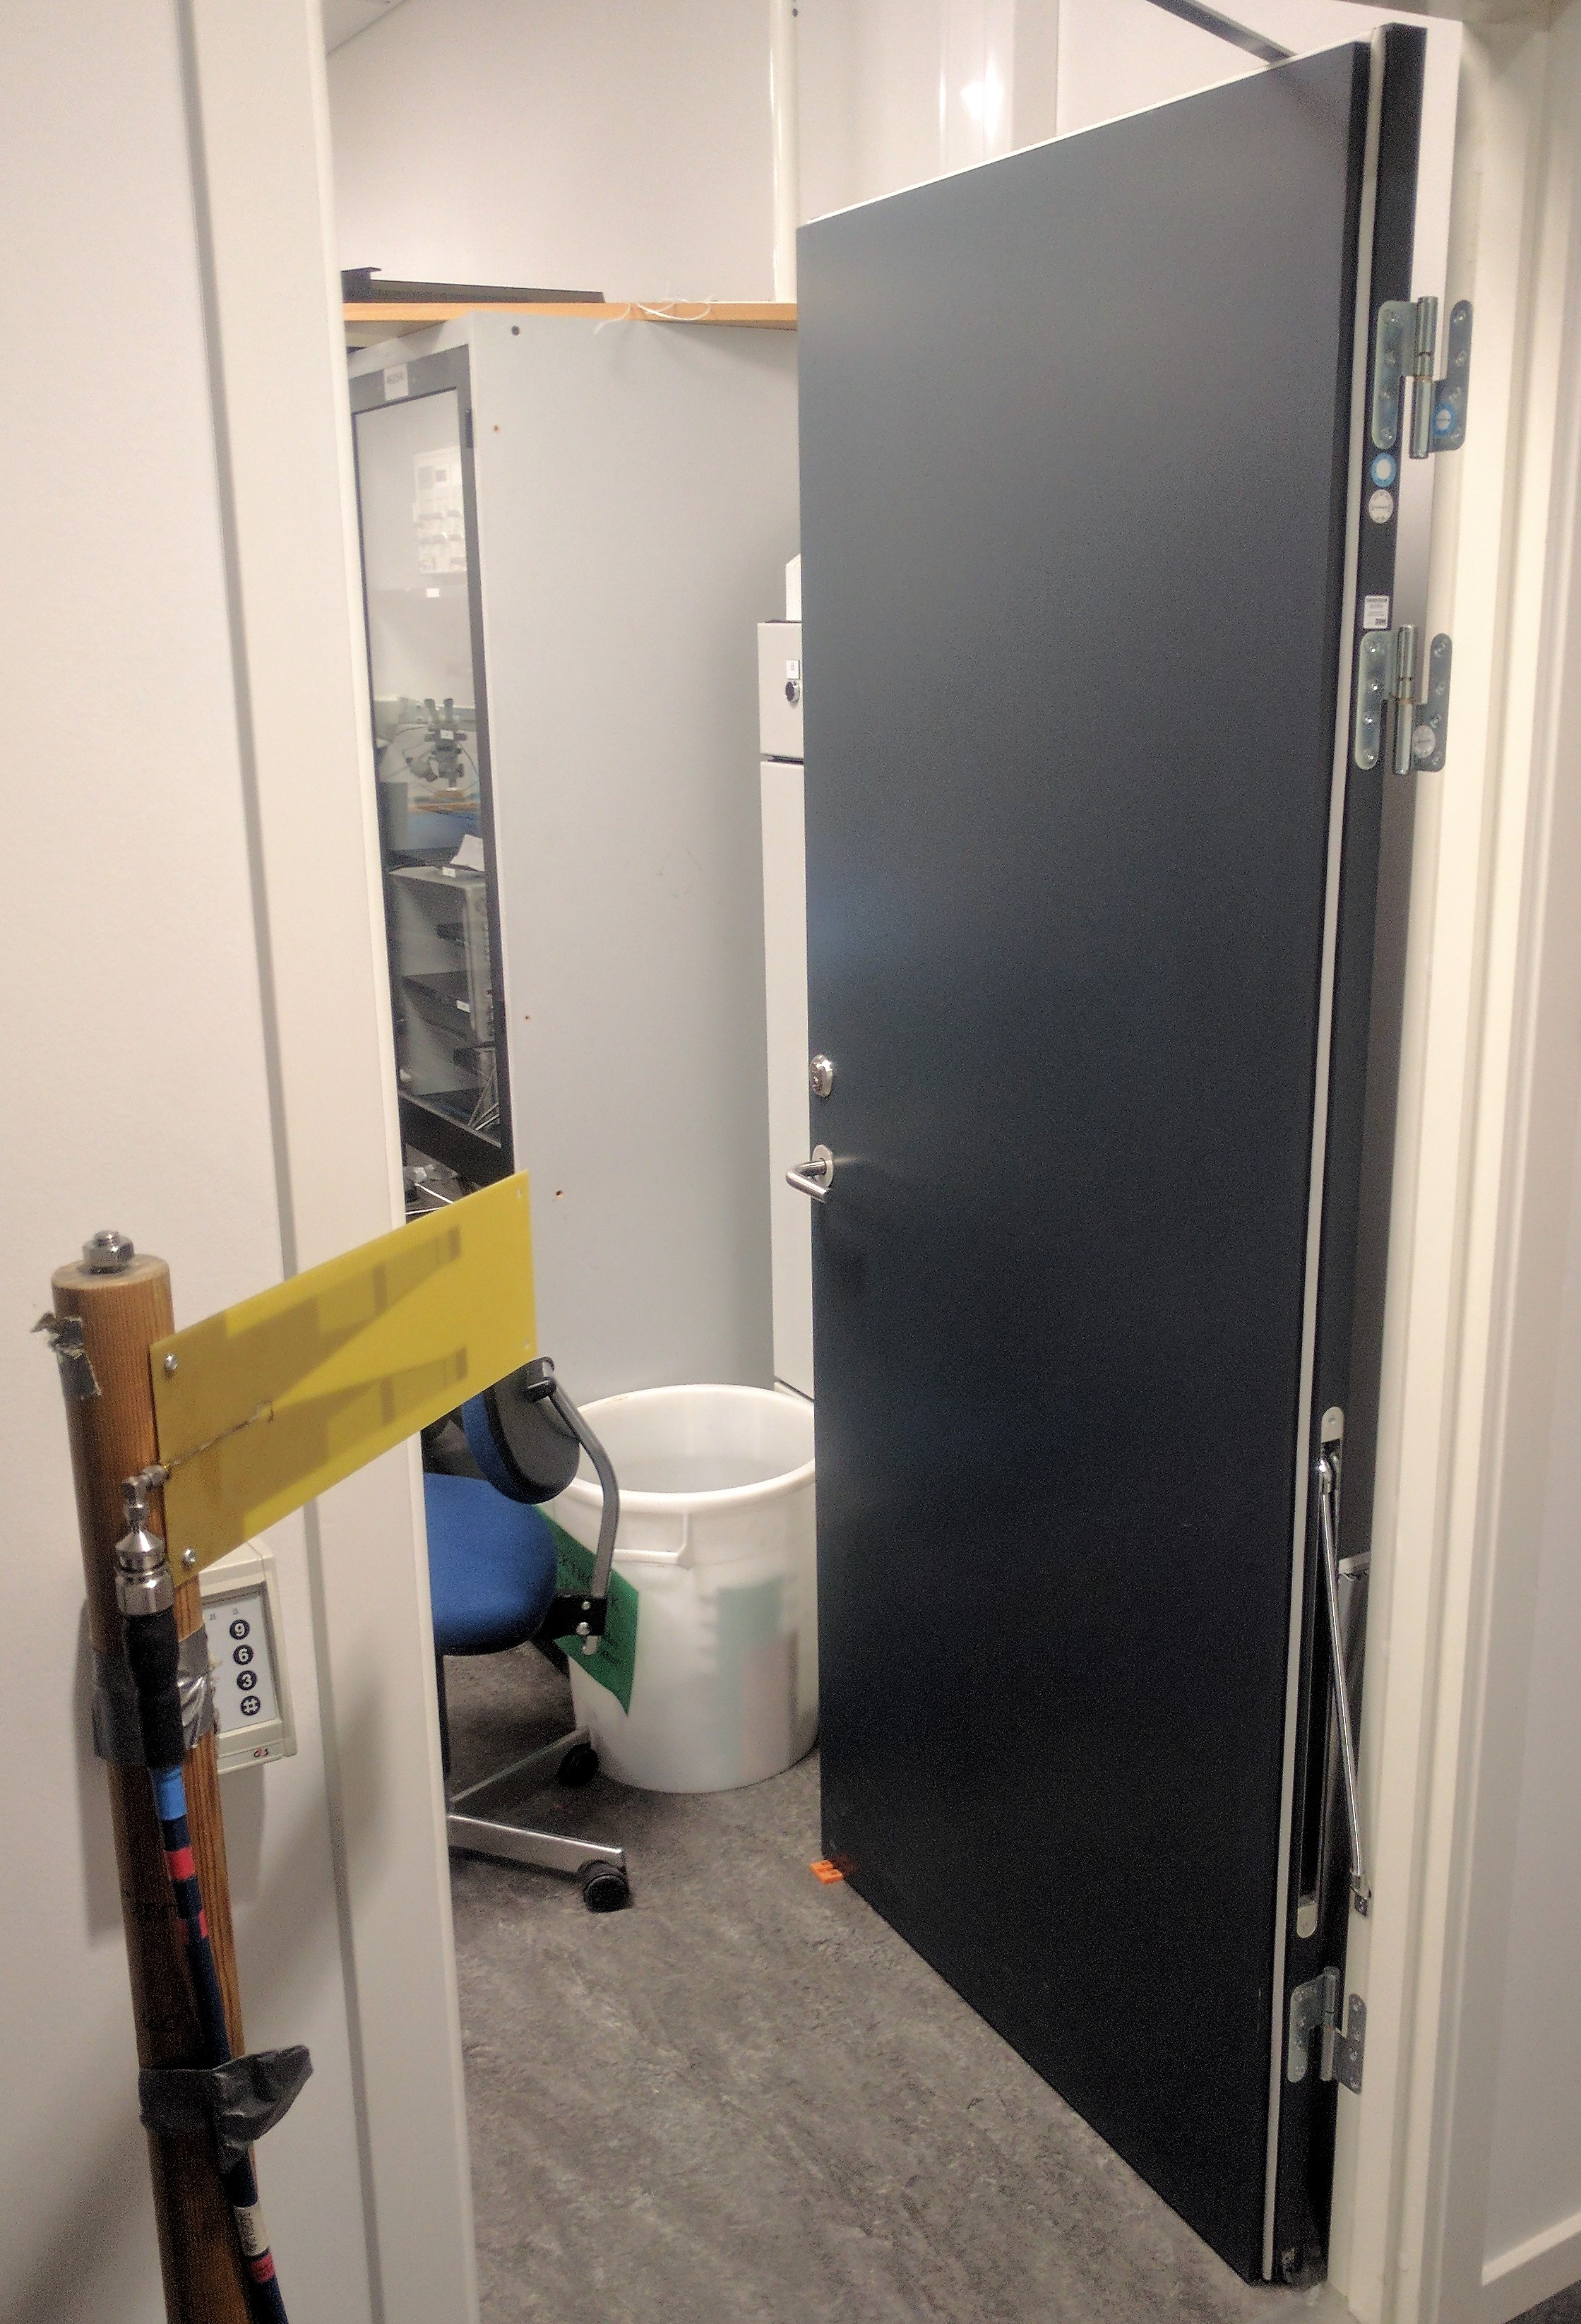
\includegraphics[width=\textwidth]{pictures/Measurement/antenna_door.jpg}
    \caption{TX antenna placement, pointing towards the door.}
    \label{antennadoor}
  \end{minipage}
  \hfill
  \begin{minipage}[H]{0.4\textwidth}
    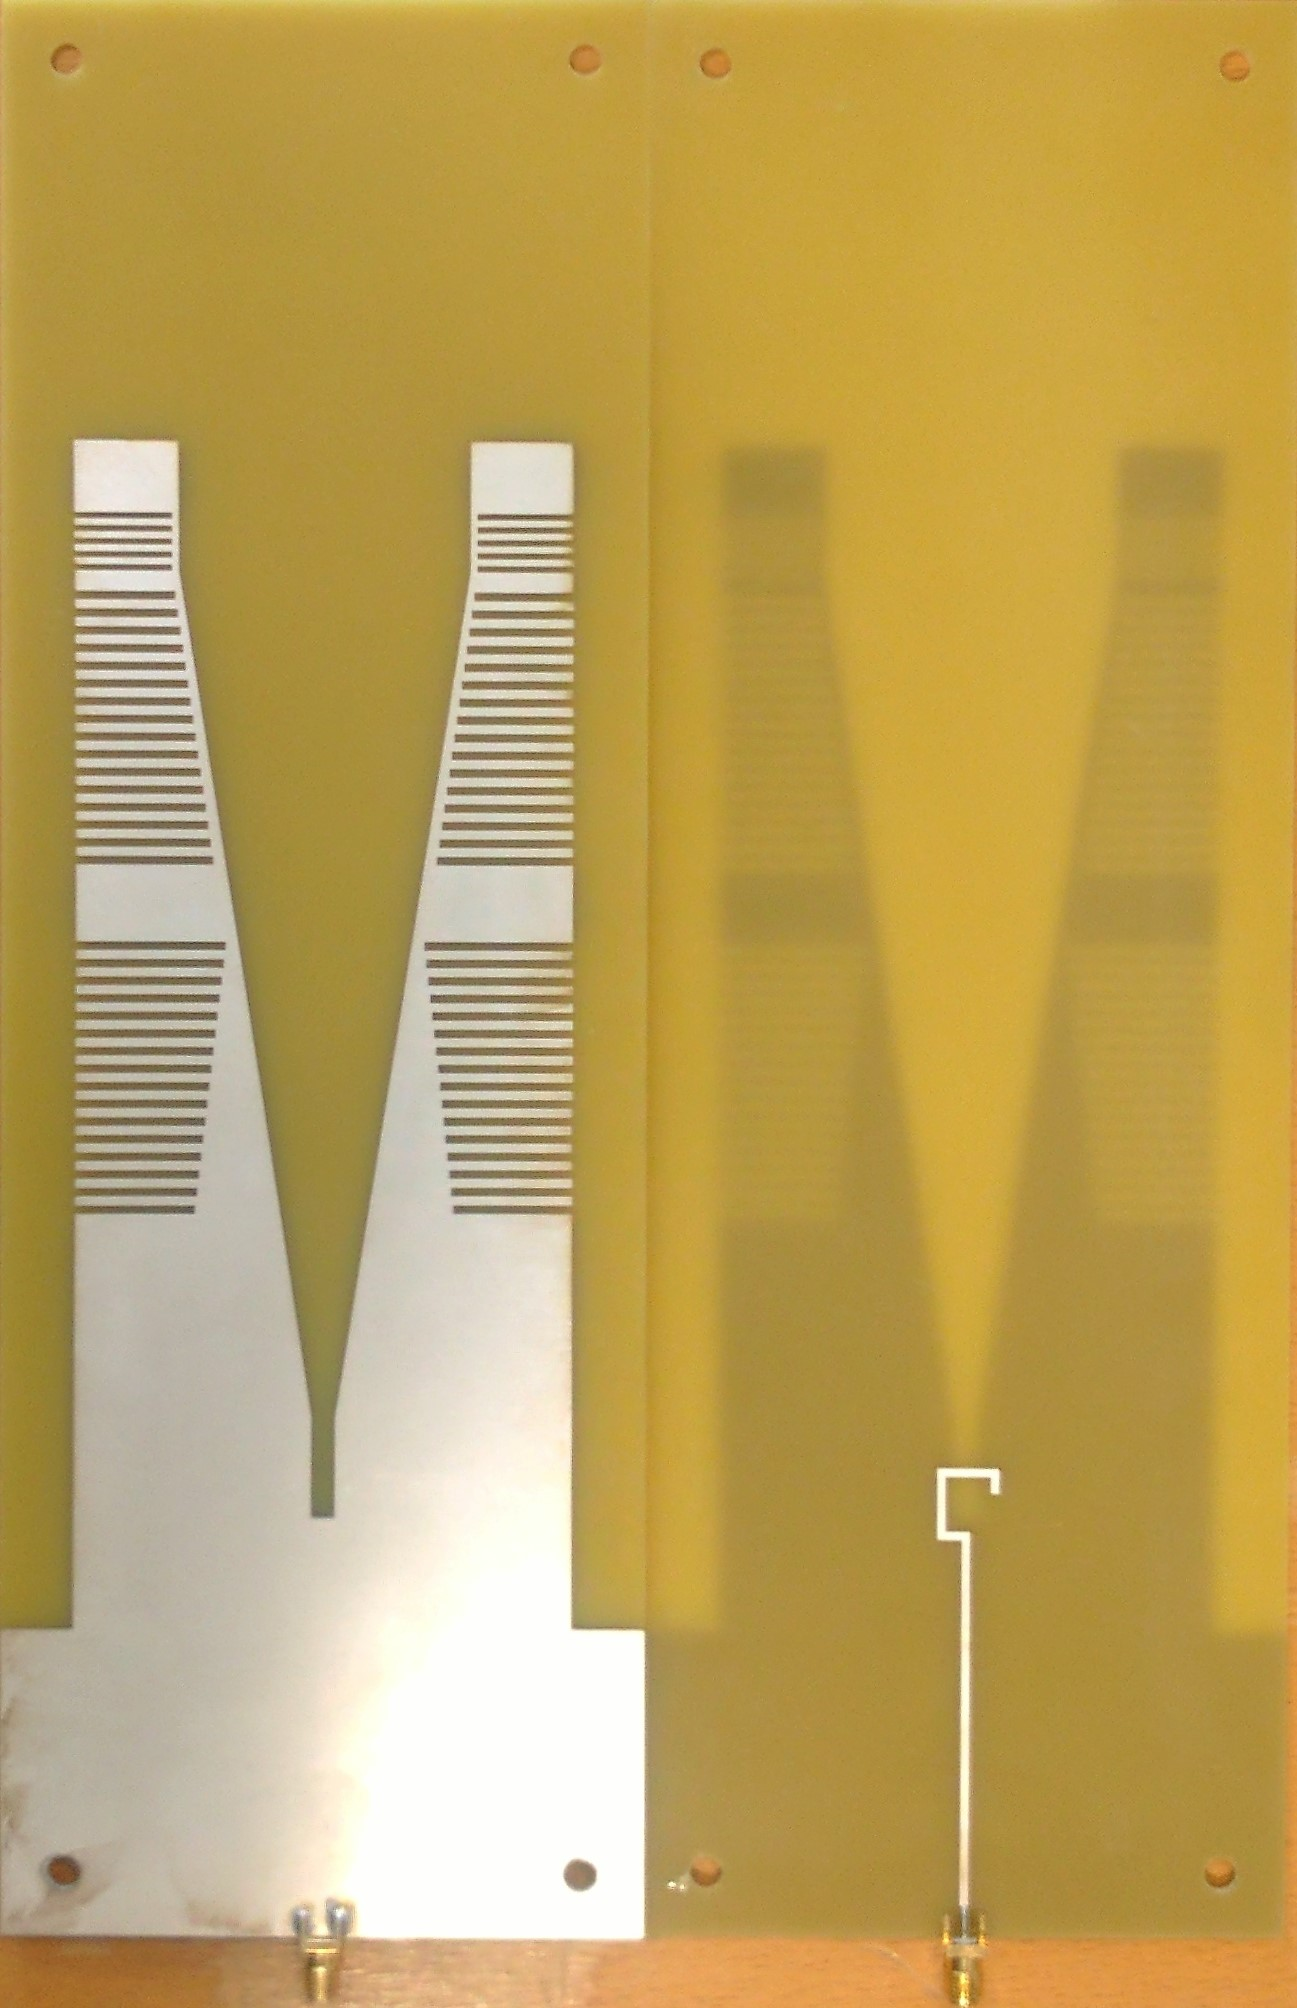
\includegraphics[width=\textwidth]{pictures/Measurement/dirrecional_antenna.jpg}
    \caption{Both sides of the directional TX antenna up close.}
    \label{DirAnt}
  \end{minipage}
\end{figure}

\begin{figure}[H]
\centering
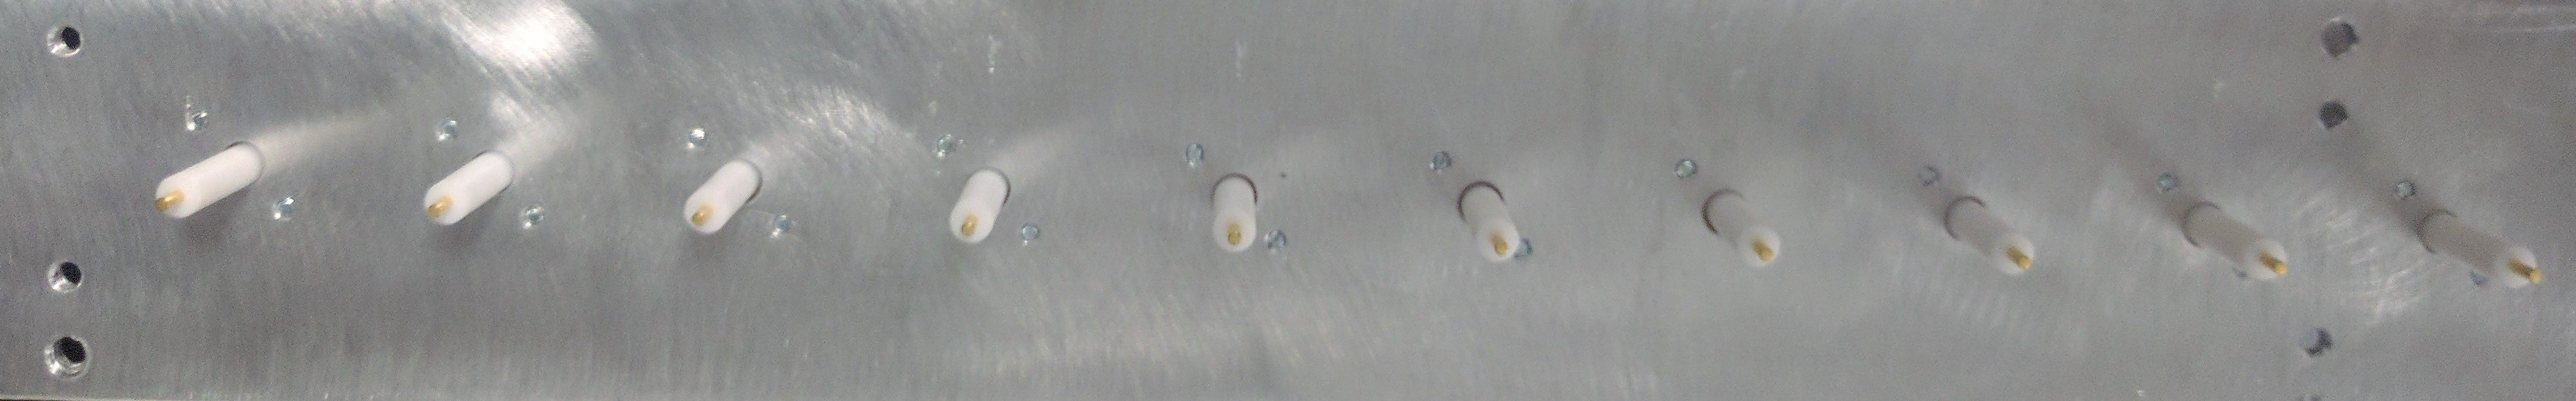
\includegraphics[width=0.7\textwidth]{pictures/Measurement/antenna_array.jpg}
    \caption{Omnidirectional RX antenna array with $0.4 \lambda$ spacing}
    \label{OmniDirAnt}
\end{figure}




\subsection{Connected setup}
\label{connected_setup}

\begin{figure}[H]
\centering
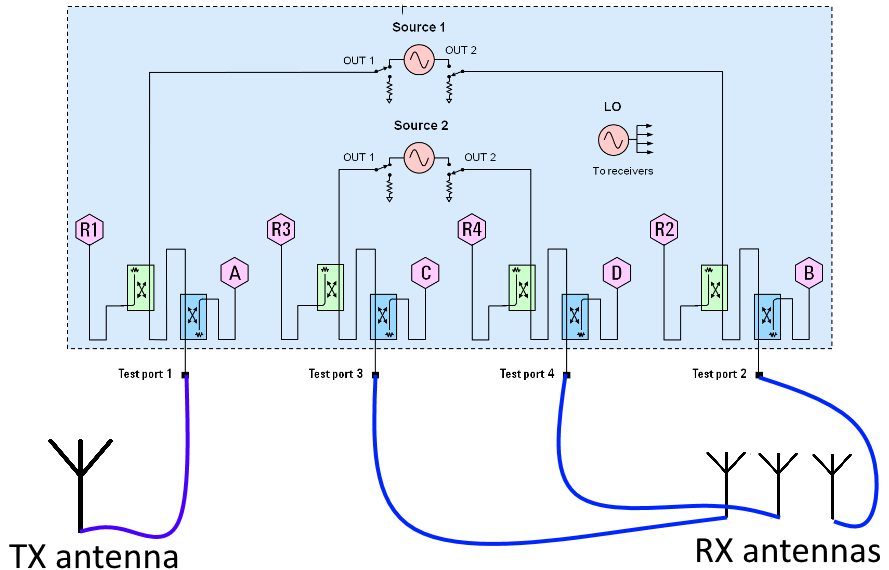
\includegraphics[width=0.65\textwidth]{figures/Gimp_figures/4portVNA.png}
\caption{VNA connections \citep{Key_PNA}}
\label{connection_diagram}
\end{figure}

The RX antennas was connected directly to the VNA before the coupling (blue box in \autoref{connection_diagram})to reduce the attenuation. After setting up everything we found out that $P_{RX}$ was lower then expected. To increase the $P_{RX}$ the TX antenna was moved closer to the door and a shorter cable was used, this can be seen \autoref{antennadoor}. The NLOS condition was still fulfilled. 

%Keysight PNA N5527A 4-port VNA with parallel measurements and supports a frequencies from 10MHz to 67 GHz. The sweep data will me saved to a USB.
%
%Cables used have a loss of $0.5dB per m$ 
%Splitter to separate the signal to two TX antennas and point towards the doors for more equal distribution of signal.
%N5527A has a $-119dB$ noise floor without averaging with a 10Hz $IF_{bw}$ at 1-10GHz. The dynamic range of the VNA becomes:
%
%\begin{equation}
%DR = P_{tx}-119dBm 
%\label{NFvna}
%\end{equation}


%The most important part of the setup is the equipment and how they are connected. The R\&S Spectrum Analyser (model FPL9KHz-6GHz) is the center of the setup. This is the receiver of our system and gives us a readout of the spectrum in terms of power (dBm) and frequency (Hz). The two main setting on the Spectrum analyser is IF filter bandwidth and resolution. These two values gives us a sweep time.
\chapter{Setup Parameter estimation}\label{sec:setup_parameter}
Before staring measuring the settings on the VNA needs to be determined. This means that the values has to be  balanced to get the needed data and to meet the physical limitations. Part I goes thorough the theory and the limiting factors has been discussed.

\todo{parameters we set: Tx power, Span, Center frequency, IFbw, Nsweep}


\section{TX power}
The transmit power $P_{TX}$ is the maximum power the VNA can transmit without getting overloaded. This should be as high as possible but given that a \gls{PA} is not used this should be around 15dBm \citep{Key_PNA} depending on load from the different antennas and the VNA.

